\documentclass{beamer}
\usetheme[color=ACMblue]{ACMNew}
\usepackage{beamernotes}
\usepackage{algpseudocodex}
\usepackage{lipsum}
\usepackage{minted}
\usepackage{array}
\usepackage{tikz}
\usepackage{amsmath}
\usepackage{mathtools}
\usepackage{xcolor}
\usemintedstyle{manni}
\pdfcompresslevel=9
\pdfobjcompresslevel=3

\title[ACM fun]{CS 374B Review MT3}
\subtitle{Turing Complete Spookiness}
\author{ACM @ UIUC}
% \institute{The Mental Institute}  
\date{November 3, 2024}

\begin{document}

\begin{frame}
  \titlepage
\end{frame}
\bnote{This generates notes for pdfpc. These notes also appear
  on the handout/article versions.}

\begin{frame}[t]{Disclaimers and Logistics}
  \begin{itemize}
  \item \alert{Disclaimer:} Some of us are CAs, but we have not seen the exam. We have no idea what the questions are. However, we've taken the course and reviewed Kani's previous exams, so we have \alert{suspicions} as to what the questions will be like.
  \item This review session is being recorded. Recordings and slides will be distributed on EdStem after the end.
  \item \alert{Agenda:} We'll quickly review all topics likely to be covered, then go through a practice exam, then review individual topics by request.
  \begin{itemize}
      \item Questions are designed to be written in the same style as Kani's previous exams but to be \textit{slightly} harder, so don't worry if you don't get everything right away!
  \end{itemize}
  \item Please let us know if we're going too fast/slow, not speaking loud enough/speaking too loud, etc.
  \item If you have a question anytime during the review session, please ask! Someone else almost surely has a similar question.
  \item We'll provide a feedback form at the end of the session.
  \end{itemize}
\end{frame}

\begin{frame}[t]{P and NP}
% "Ability to prove that a given problem is in NP" is on the skillset
    \begin{itemize}
        \item A \alert{decision problem} is a problem with a true/false answer. (yes/no, etc.)
        \item \alert{P} is the set of decision problems with a polynomial-time solver.
        \item \alert{NP} is the set of decision problems with a polynomial-time \emph{nondeterministic} solver.
        \item Alternatively, NP is the set of decision problems with a polynomial-time \emph{certifier} for "true" answers, given a polynomial-size \emph{certificate}.
        \begin{itemize}
            \item Intuitively, with an NP problem, we can verify a "yes" answer quickly if we have the solution in front of us.
        \end{itemize}
    \end{itemize}

    \vspace{0.5em}
    \pause

    For example, consider the yes/no problem of deciding whether a graph $G = (V, E)$ has a path containing all its vertices. (Hamiltonian Path)
    \begin{itemize}
        \item If you were given the path already ($O(V)$ length) as a certificate, you could certify that the answer is "yes" in polynomial time.
        \item Therefore, this problem is in NP.
    \end{itemize}

    \vspace{0.5em}
    \pause

    Formally, an algorithm $C$ is a certifier for problem $X$ when $s \in X$ if and only if there exists string $t$ such that $C(s,t)=\text{true}$.
    \begin{itemize}
        \item $t$ here is a "certificate."
        \item We can show $X$ is NP by providing this information, and showing $C$ is polynomial-time and $t$ is polynomial-size (with respect to the size of the input $s$).
    \end{itemize}

    % we should mention Co-NP, NP-complete and NP-hard, as there's sometimes questions of the form "choose what complexity classes this problem is in" but this looks good

\end{frame}

\begin{frame}[t]{co-NP}
    \begin{itemize}
        \item \alert{co-NP} is the set of decision problems $X$ whose complements  $\overline{X}$ are in NP.
        \item Alternatively, NP is the set of decision problems with a polynomial-time certifier for \textbf{"false"} answers, given a polynomial-size certificate.
        \item For example, the problem of deciding whether a graph \emph{doesn't} have a Hamiltonian path is in co-NP.
    \end{itemize}
    co-NP isn't on your skillset, but be aware that this is \emph{not} the same thing as NP.
\end{frame}

\begin{frame}[t]{Reductions I: Intuition}
    \begin{itemize}
        \item \alert{Intuition:} Problem $B$ is ``at least as hard'' than problem $A$ if we can use a black-box problem $B$ solver ($B$ oracle) to solve problem $A$ with limited overhead (generally, polynomial-time).
        \item \pause We know a variety of ``hard'' problems, so if we want to show that a problem $B$ is hard, we need to show that oracles can be used to quickly solve some hard problem $A$ (even if we believe that that oracle doesn't exist!). This is building a \alert{reduction from} problem $A$ \alert{to} problem $B$
        \item \pause A problem is \alert{NP-hard} if the existence of a polynomial-time algorithm for that problem would imply the existence of a polynomial-time algorithm for any problem in NP. We'll prove that problems are NP-hard by providing \alert{polynomial-time} reductions from a known NP-hard problem to the problem in question.
        \begin{itemize}
            \item \alert{NP-complete} problems are NP and NP-hard.
        \end{itemize}
        \item \pause A problem is \alert{undecidable} if \textit{no} algorithm exists that always completes in the right answer.  We'll prove that problems are undecidable by providing reductions from a known undecidable problem to the problem in question.
        \pause \begin{alertblock}{Make sure you're going in the right direction!}
            If you're trying to prove that a problem is NP-hard or undecidable, you need to reduce \textbf{from} an NP-hard/undecidable problem \textbf{to} the problem you want to prove is hard (in other words, show that an oracle for your problem can be used to solve an NP-hard/undecidable problem). The most common mistake on exams is reducing in the wrong direction.
        \end{alertblock}
    \end{itemize}
\end{frame}

\begin{frame}[t]{Reductions II: Tutorial}
    \begin{itemize}
        \item To show a problem is NP-hard/undecidable you need to do the following:
        \begin{enumerate}
            \item \pause Consider an oracle for the problem that you're reducing to. If you're showing that something is NP-hard, you should assume that the oracle is polynomial-time
            \item  \pause Provide an algorithm for the problem that you're reducing to using the problem that you're reducing from.
            \item \pause Analyze the runtime for your algorithm, and show it is within your target.
            \item \pause Provide a proof of correctness.
        \end{enumerate}
        \item \pause We're mostly going to be talking about \alert{decision variants} of problems (where you only need to return YES/NO) since the main complexity classes are defined with respect to them, and since, usually, decision variants are equally hard as their calculation equivalents
    \end{itemize}
    \pause \begin{exampleblock}{Template- Reduction}
    Assume that there exists an oracle function $B$ which runs in [TIME CONSTRAINT]. Thus, we can solve $A$ as follows:
            \begin{algorithmic}[1]
                \Procedure{A}{input}:
                    \State Do some preprocessing to create instances of problem $B$
                    \State outputs $\gets$ \Call{B}{generated inputs}
                    \State Do some postprocessing on outputs to get the correct answer for $A$
                \EndProcedure
            \end{algorithmic}
            
        \end{exampleblock}
\end{frame}

\begin{frame}[t]{A Tour of NP-Hard Problems: CircuitSAT and 3SAT}
    \begin{itemize}
        \item \alert{CircuitSAT}: The ``original'' NP-complete problem. Given a boolean circuit, is there a set of inputs that makes it return \texttt{true}?
            \begin{center}
                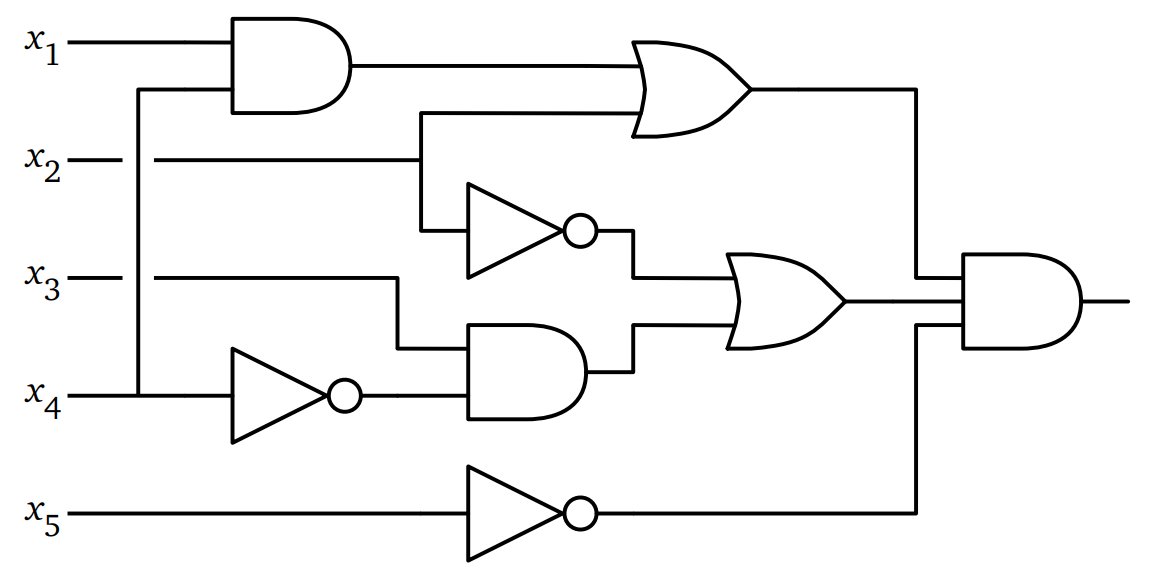
\includegraphics[height=.2\textwidth]{csat.PNG}
            \end{center}
        \item \pause \alert{3SAT}: Given a boolean formula of the form $(a \vee b \vee c) \wedge (\overline{a} \vee d \vee e) \wedge \dotsb$, is there an assignment to the input variables that makes it return \texttt{true}?
        \item \pause Consider reducing from 3SAT if$\dotsc$:
        \begin{itemize}
            \item \pause There's some structure of choice within the problem (i.e. the goal is to decide either A or B)
            \item  \pause There's a 3 in the problem, and you don't know why
        \end{itemize}
        \pause
        \begin{alertblock}{Be careful with $k$-SAT variants!}
            While $k$-SAT for $k \geq 3$ is NP-complete, there is a polynomial-time algorithm for 2SAT. (Using strongly connected components!)
        \end{alertblock}
    \end{itemize}
\end{frame}

\begin{frame}[t]{A Tour of NP-Hard Problems: CircuitSAT and 3SAT}
    Consider the problem \alert{MajSAT}: Clauses now consist of 5 literals, and you must satisfy at least 3 literals in each clause. Is \alert{MajSAT} in NP, NP-hard, both, or neither? Prove why by either stating an algorithm or providing a reduction.
\end{frame}

\begin{frame}[t]{A Tour of NP-Hard Problems: Max\{Clique, IndSet\}, MinVertexCover}
    \begin{itemize}
        \item \alert{MaxClique}: Given a graph $G$ and positive integer $h$, can we find a $K_h$ subgraph in $G$ (i.e. a set of $h$ nodes where each one has an edge to every other)?
        \pause \begin{center}
            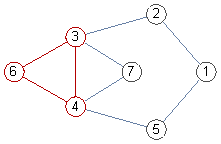
\includegraphics[width=0.22\linewidth]{clique.pdf}
        \end{center}
        \item \pause \alert{MaxIndSet}: Given a graph $G$ and positive integer $h$, can we find a set of $h$ nodes, none of which share an edge?
        \pause \begin{center}
            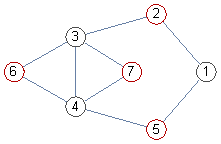
\includegraphics[width=.22\linewidth]{indset.pdf}
        \end{center}
        \item \pause \alert{MinVertexCover}: Given a graph $G$ and positive integer $h$, can we find a set of $h$ nodes so that all edges have at least one endpoint chosen?
        \pause \begin{center}
            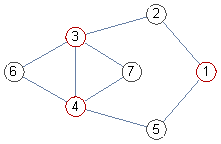
\includegraphics[width=.22\linewidth]{vtxCover.pdf}
        \end{center}
        \end{itemize}
\end{frame}

\begin{frame}[t]{A Tour of NP-Hard Problems: Max\{Clique, IndSet\}, MinVertexCover}
    ACM is writing their review session for CS/ECE 374B MT3. While making slides, each CA writes 2 problems, either alone or in collaboration with other CAs. Since all of the CAs all have inflated egos, they won't show up to the review session unless one of the problems that they worked on is in the review session. Show that determining whether we can run a review session with at most $k$ problems is NP-complete.
\end{frame}

\begin{frame}[t]{A Tour of NP-Hard Problems: Graph Coloring}
    \begin{itemize}
        \item Given an (undirected) graph, can we color the nodes with at most $k$ colors so that no two vertices that share an edge are of the same color?
        \begin{center}
            \begin{overprint}[.2\textwidth]
                \onslide<1>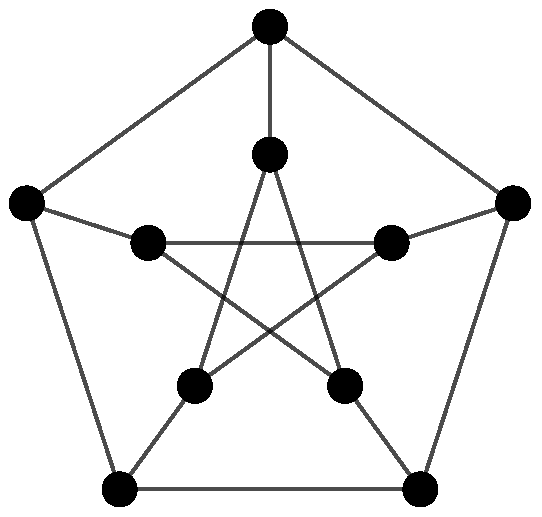
\includegraphics[width=\textwidth]{petersen.pdf}
                \onslide<2->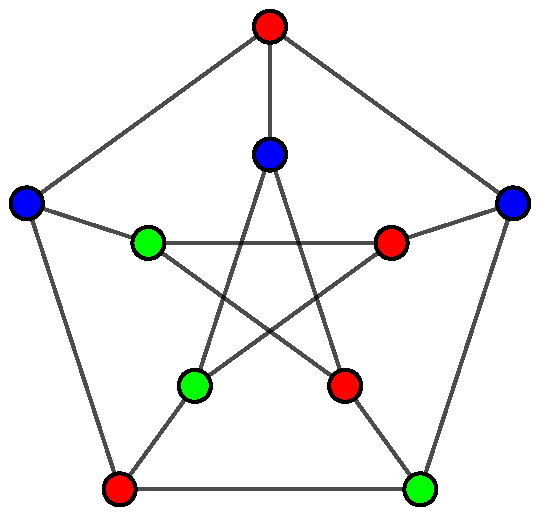
\includegraphics[width=\textwidth]{petersen_colored.pdf}
            \end{overprint}
        \end{center}
        \item \pause \pause Consider reducing from $k$-coloring if$\dotsc$:
        \begin{itemize}
             \item \pause You need to assign objects to groups, and assigning one object to a group limits your choices for some local set of others
             \item \pause There's a graph where you need to solve for some \textit{vertex} properties
        \end{itemize}
        \end{itemize}
        \pause
        \begin{alertblock}{Be careful with $k$-coloring variants!}
            While $k$-coloring for $k \geq 3$ is NP-complete, you can find whether a graph is bipartite (2-colorable) using DFS.
        \end{alertblock}
    
\end{frame}

\begin{frame}[t]{A Tour of NP-Hard Problems: Graph Coloring}
    Consider the problem \alert{Safe7Color}, which asks you to color a graph with 7 colors, such that it is a violation if there is an edge $u \leftrightarrow v$ where $c(u)$ and $c(v)$ differ by 0 or 1 (mod 7). Is this problem NP-hard?
\end{frame}

\begin{frame}[t]{A Tour of NP-Hard Problems: Hamiltonian Paths and Cycles}
    \begin{itemize}
        \item A \alert{Hamilton Path} is a path that goes through each vertex \textit{exactly} once. Likewise, a \alert{Hamiltonian Cycle} is a cycle that goes through each node \textit{exactly} once.
        \begin{itemize}
            \item Every graph with a Hamiltonian cycle has a Hamiltonian path, but not every graph with a Hamiltonian cycle has a Hamiltonian path.
        \end{itemize}
        \begin{center}
            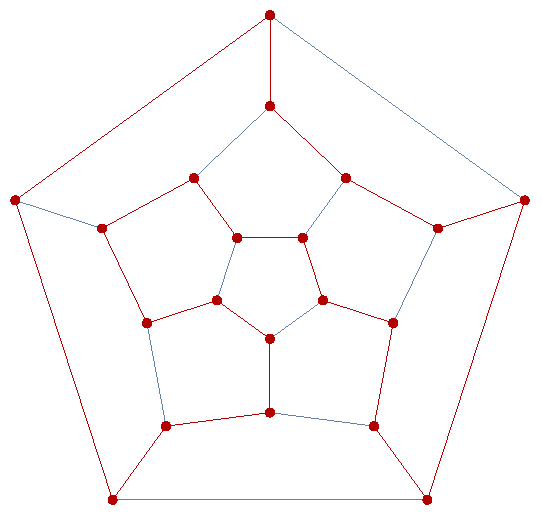
\includegraphics[height=.3\linewidth]{hamcycle.pdf}
        \end{center}
        \item \pause Consider reducing from \alert{HamPath} or \alert{HamCycle} if$\dotsc$
        \begin{itemize}
            \item \pause You're given a graph, and you're asked to find a sequence of vertices
            \item \pause You have a resource pool, and you want to use up everuthing
        \end{itemize}
    \end{itemize}
\end{frame}

\begin{frame}[t]{A Tour of NP-Hard Problems: Hamiltonian Paths and Cycles}
A \alert{balloon graph} of size $\ell$ is a cycle of length $\ell$ attached to a path of length $\ell$, where the cycle and the path are disjoint except for the connecting vertex. Show that it is NP-hard to determine whether a graph has a balloon subgraph of size at least $k$.
\begin{center}
    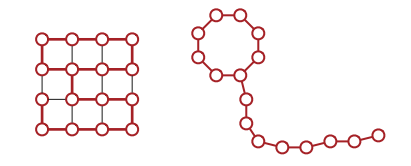
\includegraphics[width=.4\linewidth]{balloon.PNG}
\end{center}
\end{frame}

\begin{frame}[t]{A Tour of NP-hard Problems: Others}
    \begin{itemize}
        \item These likely won't come up on exams, but they're useful to know.
        \item \pause \alert{LongestPath}: given a (directed, weighted) graph $G$, is there a path of length at least $k$?
        \item \pause \alert{IntegerLinearProgramming}: given a linear objective function to optimize, as well as linear constraints, what is the largest objective achievable where (all/some) variables are restricted to integers?
        \item \pause \alert{TravelingSalesman}: given a weighted graph $G$, what is there a Hamiltonian path in $G$ of length at most $k$?
        \item \pause \alert{SubsetSum}: given a list of integers, is there a subset that sums to exactly $k$?
        \item \pause \alert{Checkers}: given a $n \times n$ checkerboard, is there a move that captures at least $k$ checkers?
    \end{itemize}
\end{frame}

\begin{frame}[t]{Undecidability}
    \begin{itemize}
        \item A language is \alert{decidable} if there exists an algorithm which always returns \texttt{true} to all inputs in $L$ and \texttt{false} to inputs not in $L$
        \begin{itemize}
            \item If we can only return \texttt{true} to all inputs in $L$ and either return $\texttt{false}$ \textit{or} infinite-loop for all other inputs, the language is merely \alert{acceptable}.
        \end{itemize}
        \begin{theorem}[Turing, 1936]
            The language \texttt{Halt}: $\{(f, w): \text{ the function } f \text{ does not infinite loop on input } w\}$ is undecidable.
        \end{theorem}
        \item 3 main ways to prove that a problem is undecidable:
        \begin{enumerate}
            \item \pause Reduce from Halt: Given an oracle for your problem, design an algorithm to decide Halt. No runtime requirement!
            \item \pause Rice's Theorem: Very powerful, basically claims that any non-trivial question about functions/Turing machines is undecidable:
            \begin{theorem}[Rice]
                Let $\mathcal{L}$ be any set of languages that satisfies the following conditions: 
                \begin{itemize}
                    \item There is a Turing machine $Y$ such that Accept($Y$) $\in \mathcal{L}$ .
                    \item There is a Turing machine $N$ such that Accept($N$) $\not\in \mathcal{L}$ .
                \end{itemize}
            Then, the language AcceptIn$(\mathcal{L}) \gets \{\langle M \rangle \mid \text{Accept}(M) \in \mathcal{L}\}$ is undecidable.
            \end{theorem}
            \item \pause Abuse the fact that you can put code into a function to derive a contradiction.
        \end{enumerate}
    \end{itemize}
\end{frame}
\begin{frame}[t]{Undecidability}
    For each of the following languages, either show that they are decidable by describing an algorithm that decides them, or show that they are undecidable by reduction and by Rice's theorem when possible.

    \begin{enumerate}[(a)]
        \item AcceptsRegular $= \left\{\langle M \rangle: M\text{'s accept set is regular}\right\}$
        \pause \item HaltsQuadratically $= \left\{\langle M \rangle, r: M \text{ halts on } r \text{ in at most } |r|^2 \text{ arithmetic operations}\right\}$
        \pause \item AcceptsRejects $= \left\{\langle M \rangle: M\text{'s accept set} = M\text{'s reject set}\right\}$
        \pause \item CFLAccepts374 $= \left\{c \in CFGs: c \text{ accepts exactly 374 strings}\right\}$
        \pause \item LeftThrice $= \left\{\langle M, w \rangle: M \text{ moves left on input } w \text{ three times in a row}\right\}$
        \pause \item NeverLeft $= \left\{\langle M, w \rangle: M \text{ never moves left on input } w\right\}$
    \end{enumerate}
\end{frame}

\begin{frame}[t]{Feedback}
    \begin{itemize}
        \item Please fill out the feedback form: \texttt{go.acm.illinois.edu/cs374b\_mt3\_feedback}\vspace{.05\textwidth}\begin{center}
            
\includegraphics[height=.5\textwidth]{feedback.pdf}
        \end{center}
    \end{itemize}
\end{frame}
\end{document}
